\documentclass[11pt]{article}

\usepackage[utf8]{inputenc}
\usepackage[margin=1in]{geometry} 
\usepackage{amsmath,amsthm,amssymb,graphicx,mathtools,tikz,hyperref,multicol,cancel,enumitem,booktabs,float,pgfplots,multirow,mathrsfs,textcomp,gensymb,soul,changepage,threeparttable}
%\usepackage[table]{xcolor}
\usepackage[T1]{fontenc}
\usepackage[italian]{babel}
\usepackage{hyphenat}
\usepackage{subfig}
\hyphenation{mate-mati-ca recu-perare}
\usetikzlibrary{positioning}
\pgfplotsset{compat=1.14}

\newcommand{\n}{\mathbb{N}}
\newcommand{\z}{\mathbb{Z}}
\newcommand{\q}{\mathbb{Q}}
\newcommand{\cx}{\mathbb{C}}
\newcommand{\real}{\mathbb{R}}
\newcommand{\field}{\mathbb{F}}
\newcommand{\ita}[1]{\textit{#1}}
\newcommand{\com}[2]{#1\backslash#2}
\newcommand{\oneton}{\{1,2,3,...,n\}}
\newcommand{\idea}[1]{\begin{gather*}#1\end{gather*}}
\newcommand{\ef}{\ita{f} }
\newcommand{\eff}{\ita{f}}
\newcommand{\proofs}[1]{\begin{proof}#1\end{proof}}
\newcommand{\inv}[1]{#1^{-1}}
\newcommand{\setb}[1]{\{#1\}}
\newcommand{\en}{\ita{n }}
\newcommand{\vbrack}[1]{\langle #1\rangle}
\newcommand{\qRa}{\quad \Rightarrow \quad}
\newcommand{\smaca}[1]{\textbf{\textsc{#1}}}

\newenvironment{theorem}[2][Teorema]{\begin{trivlist}
\item[\hskip \labelsep {\bfseries #1}\hskip \labelsep {\bfseries #2.}]}{\end{trivlist}}
\newenvironment{lemma}[2][Lemma]{\begin{trivlist}
\item[\hskip \labelsep {\bfseries #1}\hskip \labelsep {\bfseries #2.}]}{\end{trivlist}}
\newenvironment{exercise}[2][Esercizio]{\begin{trivlist}
\item[\hskip \labelsep {\bfseries #1}\hskip \labelsep {\bfseries #2.}]}{\end{trivlist}}
\newenvironment{proposition}[2][Proposizione]{\begin{trivlist}
\item[\hskip \labelsep {\bfseries #1}\hskip \labelsep {\bfseries #2.}]}{\end{trivlist}}
\newenvironment{corollary}[2][Corollario]{\begin{trivlist}
\item[\hskip \labelsep {\bfseries #1}\hskip \labelsep {\bfseries #2.}]}{\end{trivlist}}

\hypersetup {
    colorlinks,
    linkcolor=blue
}

\graphicspath{{img/}}

\begin{document}
\setlength{\parindent}{0pt}
\title{\vspace{-4em}{\large Laboratorio di Meccanica e Termodinamica} \\
    Relazione di Laboratorio}
\author{GRUPPO 3 \\ 
Gerardo Selce, Maurizio Liguori, Emanuela Galluccio, Francesco Messano}
\date{26/11/2024}
\maketitle

\vspace{-2em}\par\noindent\rule{\textwidth}{0.4pt}
\begin{center}
    {\Large\sc Misura del coefficiente di viscosità di un fluido}
\end{center}
\par\noindent\rule{\textwidth}{0.4pt}
\section{Introduzione}
Scopo dell'esperienza è la misurazione del coefficiente di viscosità di un fluido utilizzando il metodo della sfera cadente. Questo metodo si basa sull'osservazione del moto di una sfera che cade attraverso il fluido in condizioni di equilibrio dinamico. Quando la sfera raggiunge la velocità limite $v_l$ si può calcolare il coefficiente di viscosità $\eta$ dalla relazione:
\begin{equation}
    \eta=\frac{2}{9}R^2\frac{(p_s-p)}{v_l}g
\end{equation}
Prima effettuare l'esperimento sono state misurate le densità del fluido e delle sfere. Di quest'ultime è stato misurato anche il volume, necessario a misurare la forza d'Archimede a cui sono sottoposte nel fluido. Per la misurazione della velocità limite delle sfere abbiamo considerato la loro velocità media di caduta nel becher ripieno di liquido.

\section{Richiami teorici}
Si consideri un corpo di massa $m$ che cade, sotto l'azione della forza peso, in un mezzo fluido. Le forze agenti sono la forza peso $\vec{F_p}$, la spinta di Archimede $\vec{F_A}$, e la forza di attrito viscoso $\vec{F_v}$. Per un corpo di forma sferica ed in regime di moto laminare (i vari strati del fluido si muovono di moto traslatorio, senza formare vortici) la forza $\vec{F_v}$ è esprimibile nella forma:
\begin{equation}
    \vec{F_v}=-\beta\vec{v} 
\end{equation}
in cui il coefficiente di proporzionalità $\beta$ dipende dalla natura del mezzo e dalle dimensioni e forma del corpo, per un corpo sferico:
\begin{equation}
    \beta=6\pi R\eta
\end{equation}
in cui
\begin{itemize}
    \item $\mathbf{R}$ è il raggio della sfera;
    \item $\mathbf{\eta}$ è il coefficiente di viscosità del mezzo nel quale il corpo si sta muovendo.
\end{itemize}
Tenendo conto della Legge (3), la Legge (2) si scrive:
\begin{equation}
    \vec{F_v}=-6\pi R\eta
\end{equation}
\subsection{Legge di Stokes per il moto laminare}
Si consideri una sfera di raggio $R$ che cade in un fluido di densità $\rho$ e coefficiente di viscosità $\eta$ e scriviamo la sua equazione del moto:
\begin{equation}
    m\vec{a}=\vec{F_p}+\vec{F_A}+\vec{F_v}
\end{equation}
\begin{equation}
    m\frac{dv}{dt}=mg-Mg-\beta v
\end{equation}
dove $Mg$ è il modulo della spinta di Archimede, ossia il peso di liquido spostato dal corpo. Il secondo membro della Legge (6) è costituito da un termine costante $(m-M)g$ positivo ed un termine negativo (l'attrito viscoso) che cresce con la velocità. Quando questo termine negativo diventa uguale al termine costante l'accelerazione si annulla e la sfera si muove di moto uniforme con velocità pari alla velocità limite $v_l$. L'accelerazione diminuisce con il tempo fino ad annullarsi in corrispondenza della velocità limite:
\begin{equation}
    m\frac{dv}{dt}=0 \implies mg-Mg-\beta v_l=0
\end{equation}
Quindi definiamo la velocità limite:
\begin{equation}
    v_l=\frac{m-M}{\beta}g
\end{equation}
Detta $\rho_s$ la densità della sfera e $\rho$ la densità del liquido, risulta:
\begin{equation}
    m=\rho_s\frac{4}{3}\pi R^3, \ \ \ \ M=\rho\frac{4}{3}\pi R^3
\end{equation}
Inserendo questi risultati nella Legge (8) e tenendo conto della Legge (3) si ricava
\begin{equation}
    v_l=\frac{4}{3}\pi R^3\frac{(\rho_s-\rho)}{6\pi\eta R}g
\end{equation}
Da cui otteniamo la Legge (1). Le dimensioni dell'oggetto in caduta nel fluido devono essere piccole rispetto alle dimensioni del recipiente contenente il liquido, per evitare effetti dovuti alle pareti del recipiente. In paricolare, per una sfera di raggio $R$ che si muove lungo l'asse di un cilindro di raggo $R_c$ se questa condizione non è soddisfatta, occorre introdurre un fattore di correzione nella Legge (3):
\begin{equation}
    \beta=6\pi R\eta\left(1+2.4\frac{R}{R_c}\right)
\end{equation}
Pertanto:
\begin{equation}
    \eta=\frac{2}{9}R^2\frac{(\rho_s-\rho)}{v_l}g\left(\frac{1}{1+2.4\frac{R}{R_c}}\right)
\end{equation}

\section{Apparato sperimentale}
Per svolgere quest'esperienza è stato usato il seguente apparato sperimentale:
\begin{itemize}
    \item Due becher cilindrici graduati;
    \item Detersivo per piatti;
    \item Piccole sfere;
    \item Cronometro digitale;
    \item Bilancia digitale;
    \item Metro a nastro;
    \item Micrometro analogico;
\end{itemize}
\begin{table}[H]
\centering
\begin{tabular}{|c|c|}
\hline
\textbf{Strumenti di misura} & \textbf{Risoluzione} \\
\hline
Metro a nastro & $1\ mm$ \\
Cronometro digitale & $0.01\ s$ \\
Bilancia & $0.01\ g$ \\
Micrometro analogico & $0.01\ mm$ \\
Becher piccolo & $1\ ml$ \\
\hline
\end{tabular}
\caption{Risoluzione degli strumenti di misura utilizzati}
\label{tab:}
\end{table}

\begin{figure}[H]
  \centering
  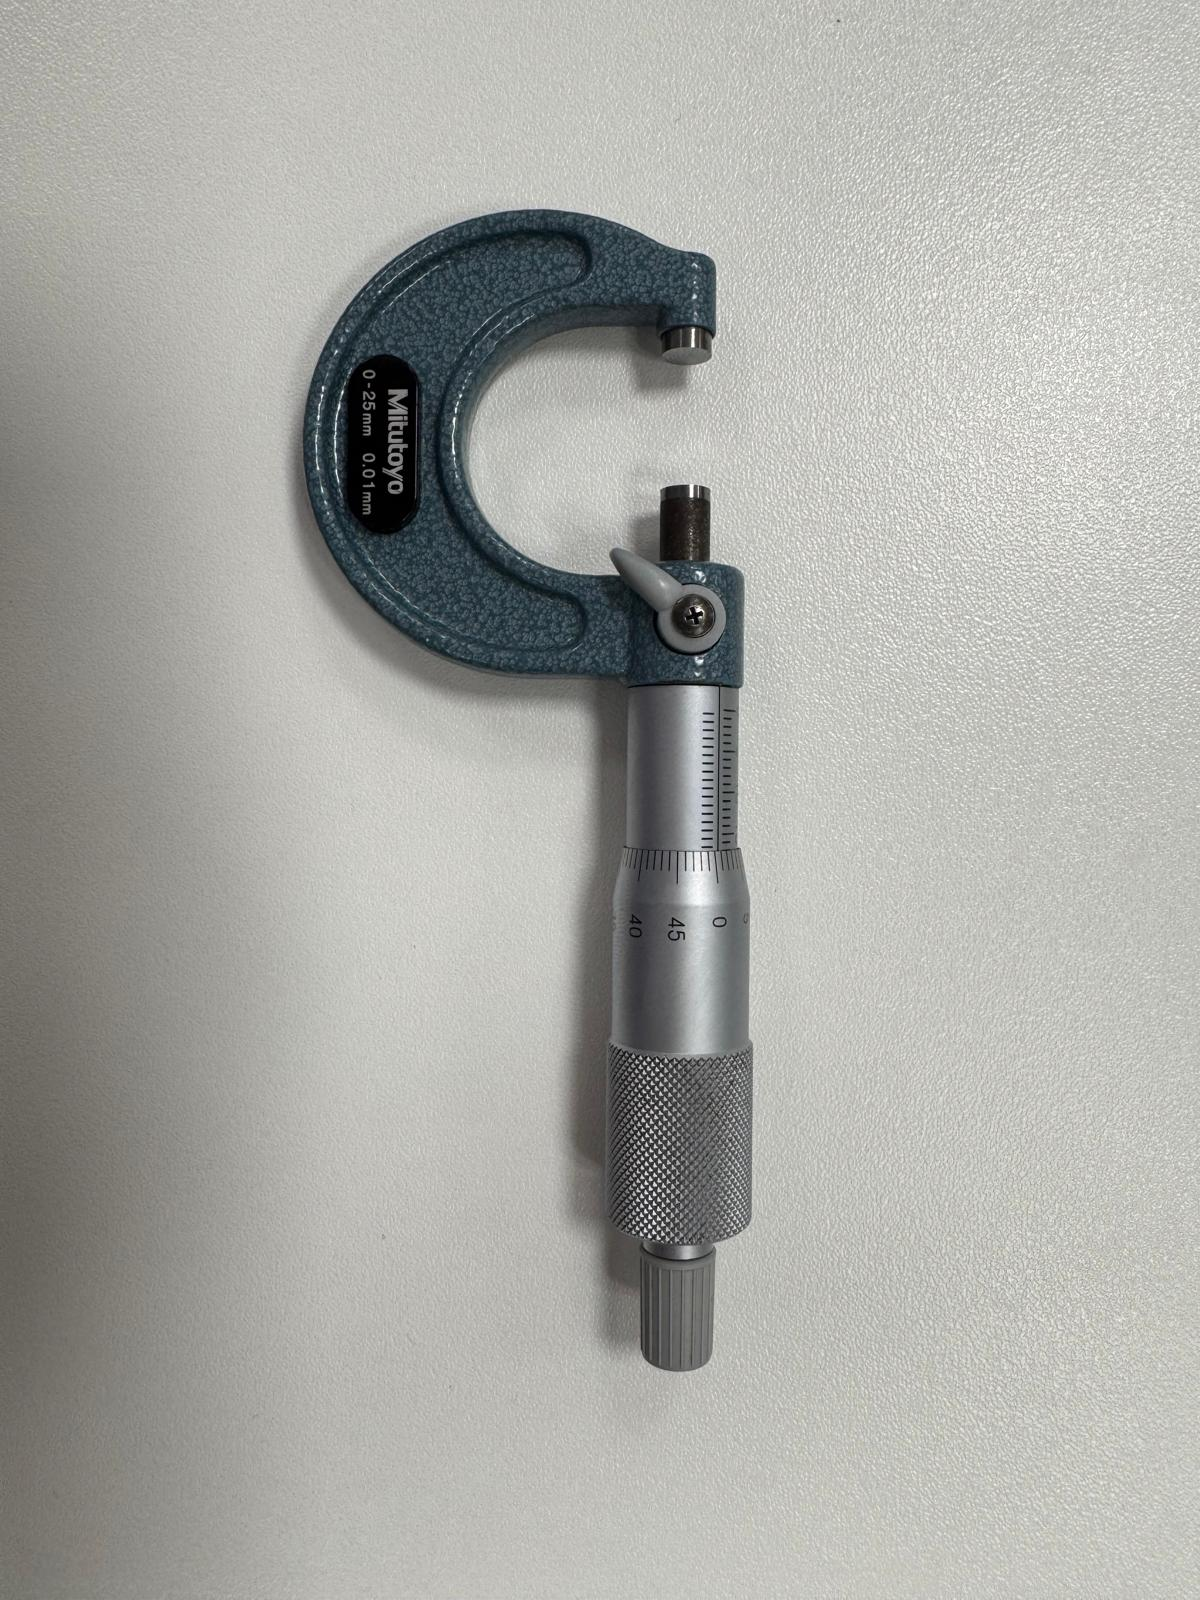
\includegraphics[width=0.55\textwidth]{micrometro.jpg}
  \caption{Micrometro utilizzato per la misurazione del diametro delle palline.}
\end{figure}

\begin{figure}[H]
  \centering
  \subfloat[Becher dentro il quale abbiamo fatto cadere le palline.]{%
    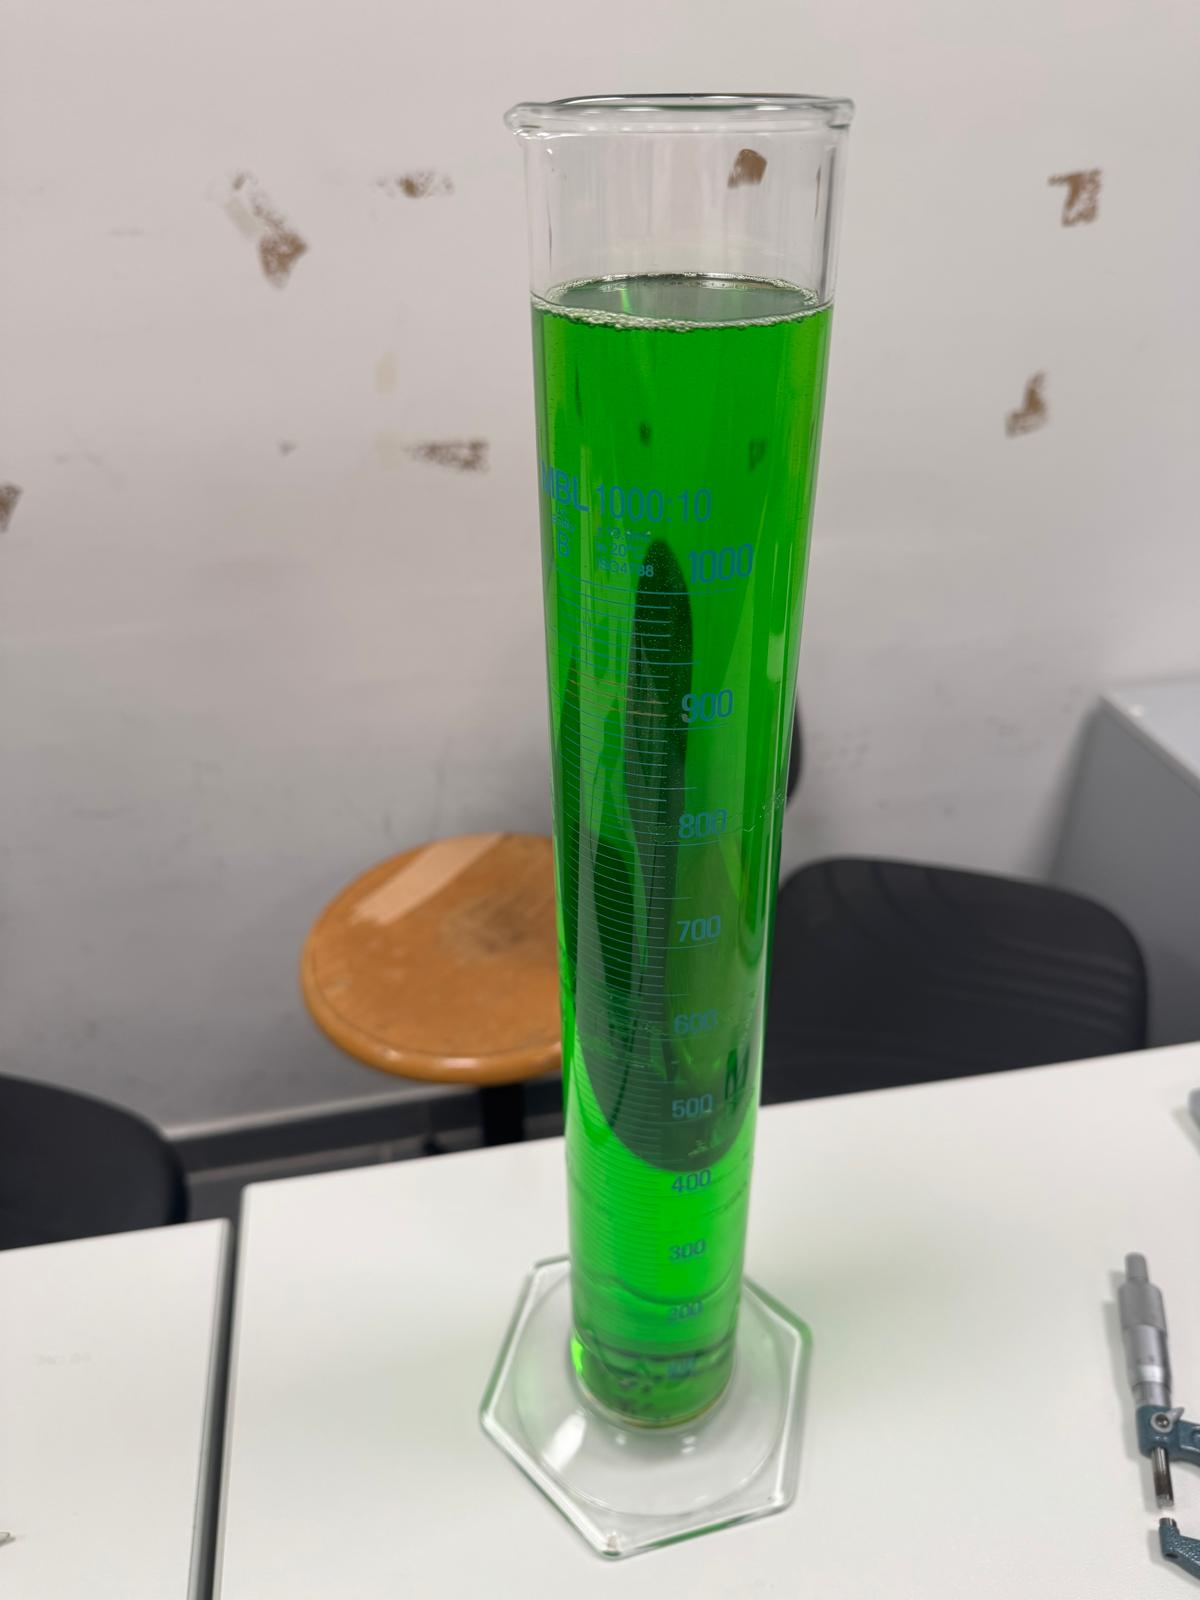
\includegraphics[width=0.35\textwidth]{bechergrande.jpg}
  }
  \hspace{0.5cm} % Spazio tra le due immagini
  \subfloat[Becher utilizzato per la misurazione della massa del liquido.]{%
    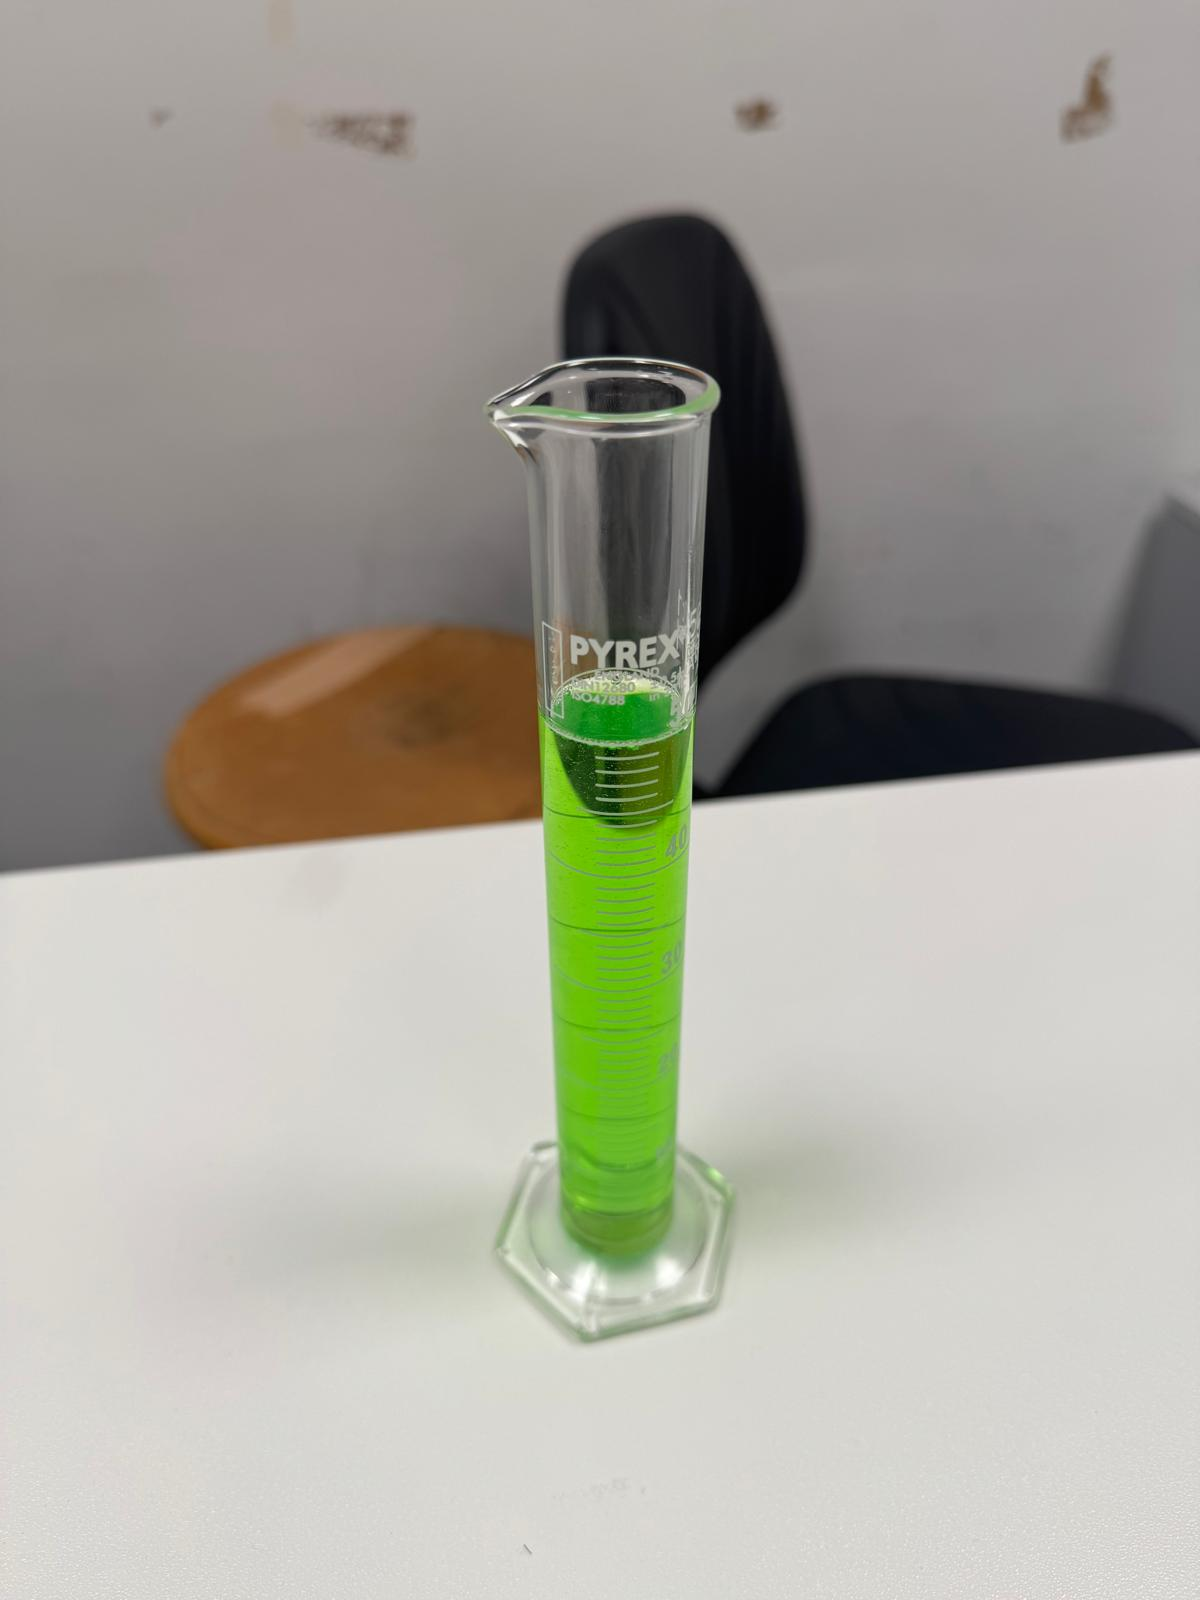
\includegraphics[width=0.35\textwidth]{becherpiccolo.jpg}
  }
  \label{fig:due_immagini}
\end{figure}

\begin{figure}[H]
  \centering
  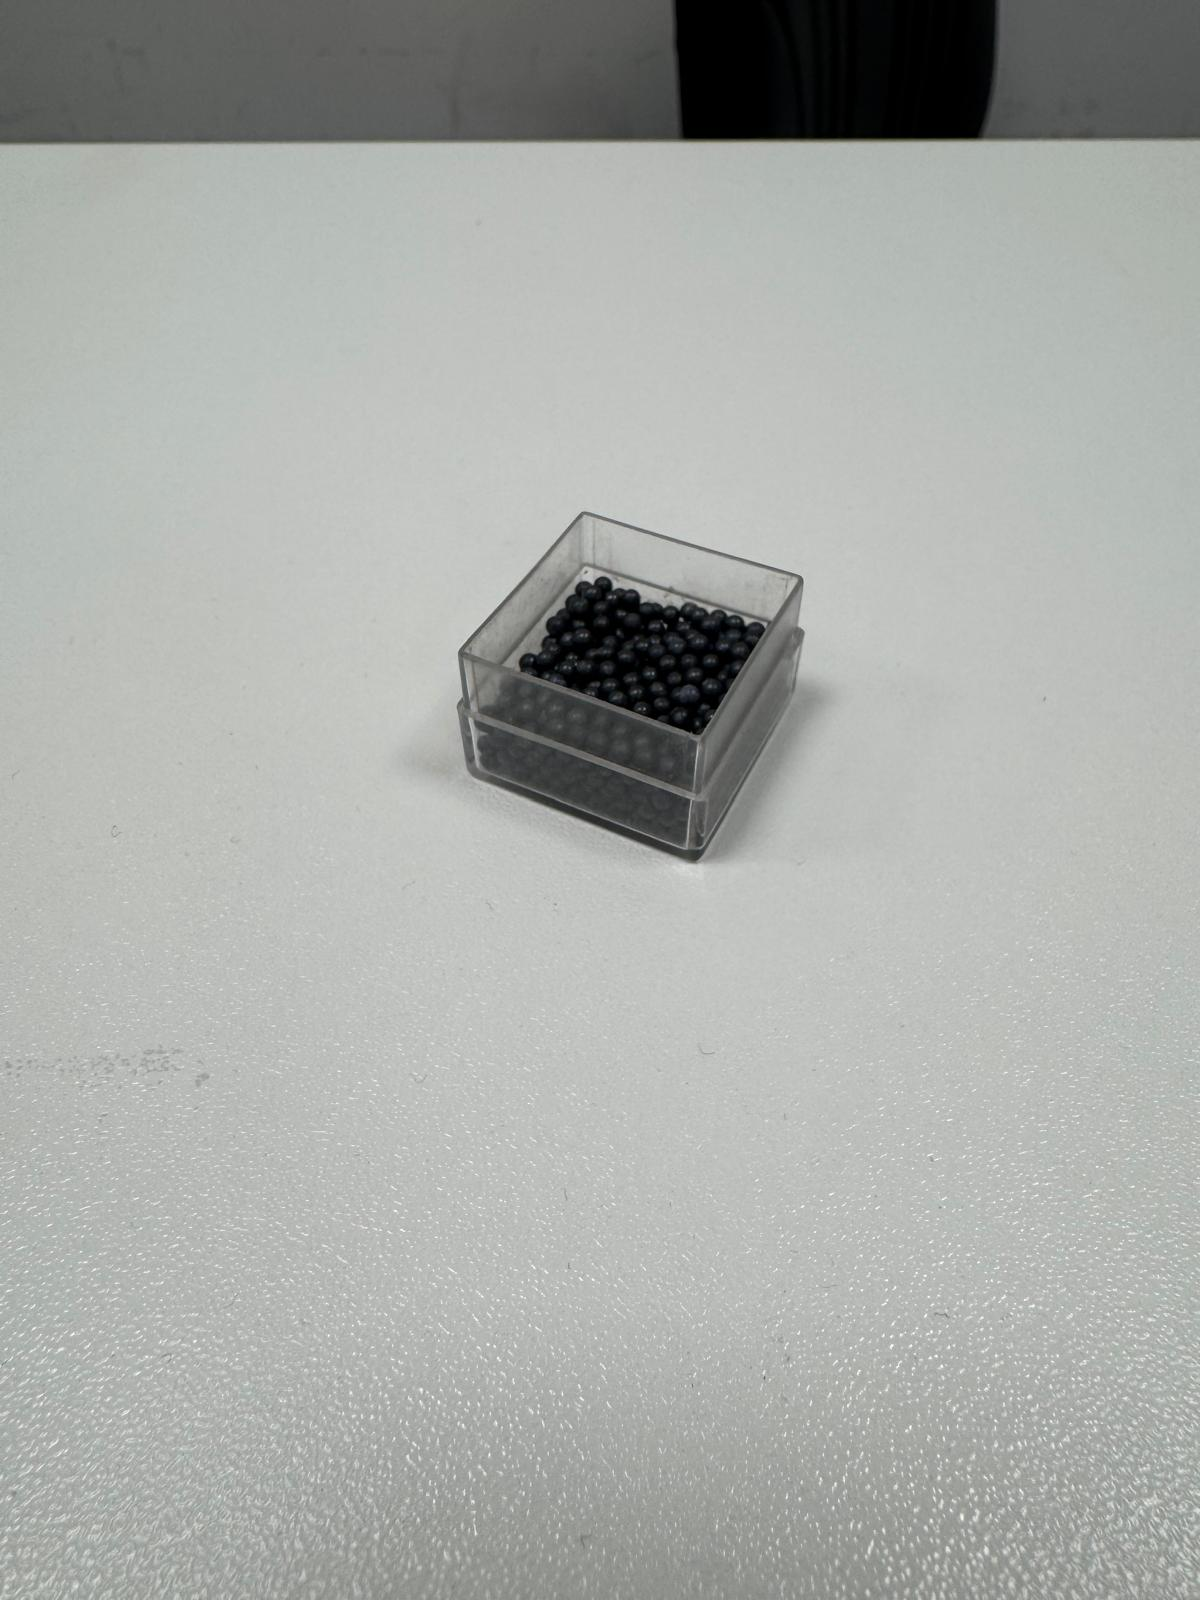
\includegraphics[width=0.55\textwidth]{palline.jpg}
  \caption{Palline usate per applicare il metodo della sfera cadente.}
\end{figure}

\section{Descrizione e analisi dei dati sperimentali}
Per il calcolo della densità delle sfere abbiamo inizialmente misurato la loro massa. Per fare ciò, abbiamo posto 50 sfere in un contenitore. La massa della singola sferetta è quindi $\frac{1}{50}$ della massa misurata, ovvero $m=(0.0692\pm 0.0004)g$. Per il calcolo del volume delle sfere sono stati misurati i diametri delle 50 sfere. Il valore finale è stato stimato come punto medio tra la misura più piccola e più grande ottenute, mentre l’incertezza sulla misura è stata valutata con la semidispersione, poichè il suo valore risulta maggiore della risoluzione strumentale. Il raggio della sfera, ovvero la metà del diametro misurato, è: $R=(1.144\pm 0.099)\ mm$.
A questo punto, considerando la formula del volume di una sfera
\begin{equation}
    V=\frac{4}{3}\pi R^3
\end{equation}
e la propagazione dell'errore 
\begin{equation}
    \Delta V = 3\frac{\Delta R}{R}V
\end{equation}
otteniamo la seguente stima del volume della singola sfera: $V=(6.2641\pm 1.6225)\ 10^{-9}\ m^3$ da cui, considerando la formula della densità
\begin{equation}
    \rho=\frac{m}{V}
\end{equation}
e la propagazione dell'errore
\begin{equation}
    \Delta \rho=\left(\frac{\Delta m}{m}+\frac{\Delta V}{V}\right)\rho
\end{equation}
otteniamo la densità:
\begin{equation}
   \rho_s=(11047\pm 2925)\frac{kg}{m^3} 
\end{equation}
Confrontando la densità ottenuta da quella di alcuni materiali noti, concludiamo che il materiale di cui sono composte le sfere è il piombo.
Per il calcolo della densità del liquido abbiamo dapprima considerato un volume noto $V=50\ ml = (5.0\pm 0.05) 10^{-5}\ m^3$. L'incertezza considerata è quella strumentale, pari alla metà della risoluzione.
Abbiamo poi misurato la massa, pari a $m=(50.03\pm 0.01)\ g$.
Dalla (15) otteniamo la densità del liquido:
\begin{equation}
    \rho = (1000\pm 20)\ \frac{kg}{m^3}
\end{equation}
Successivamente abbiamo fatto cadere le 50 sfere all'interno di questo liquido, utilizzando un becher più grande per evitare effetti dovuti alle pareti del recipiente. Abbiamo considerato lo spazio percorso dalla sfera a partire da $2cm$ dalla superficie, per un totale di
\begin{equation}
    \Delta x = (38\pm 0.05)\ cm
\end{equation}
I 50 tempi di caduta misurati sono stati raccolti in un istogramma normalizzato e ne sono state calcolate deviazione standard e media statistica, al fine da poter stimare l'intervallo in cui è contenuto il valor vero.
\begin{figure}[H]
  \centering
  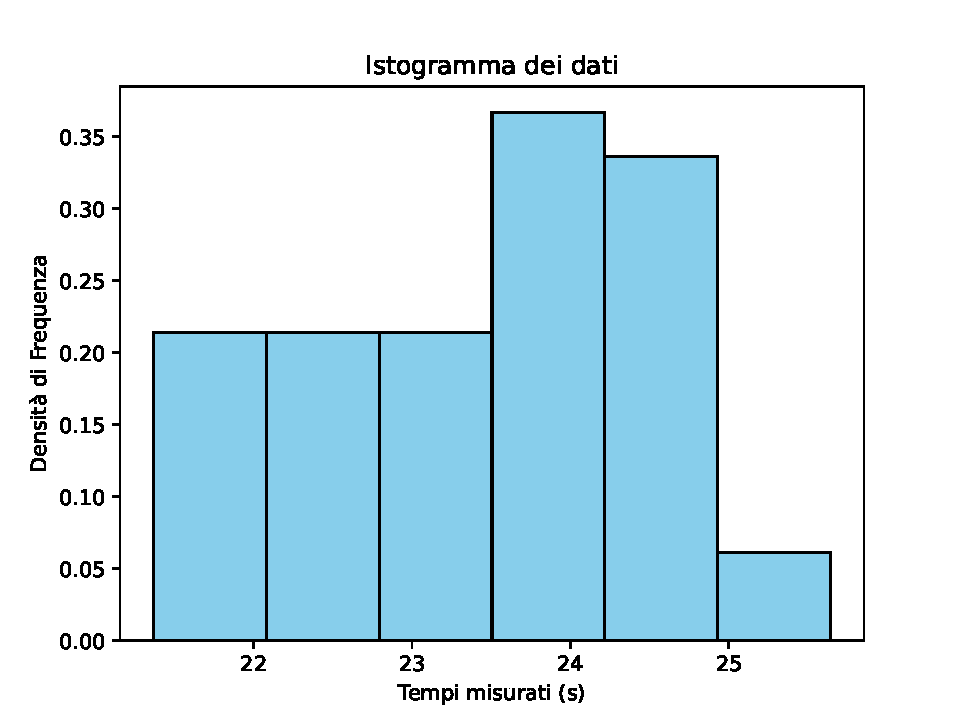
\includegraphics[width=0.85\textwidth]{istogramma.pdf}
  \caption{Istogramma normalizzato dei tempi misurati. \\
            $\mu=23.41\ s$ (Media statistica) \\
            $\xi_q=1.08\ s$ (Scarto quadratico medio) \\
            $N=50$ (Numero di campioni)}
\end{figure}
Il tempo di caduta sarà quindi uguale a:
\begin{equation}
    t=\overline{t}\pm \Delta t
\end{equation}
Con
\begin{equation}
    \overline{t} = \mu
\end{equation}
\begin{equation}
    \Delta t= 3\frac{\xi_q}{\sqrt{N}}
\end{equation}
Ovvero
\begin{equation}
    t=(23.41\pm 0.46)\ s
\end{equation}
Con questi dati è possibile calcolare la velocità limite di caduta della sfera nel liquido, pari a
\begin{equation}
    v_l = \frac{\Delta x}{t}
\end{equation}
Con la relativa propagazione dell'errore
\begin{equation}
    \Delta v_l=\left(\frac{\Delta x}{x}+\frac{\Delta t}{t}\right)v_l 
\end{equation}
Ovvero
\begin{equation}
    v_l = (0.01623\pm 0.00034)\ \frac{m}{s}
\end{equation}
A questo punto, considerando la Legge (1) e la seguente propagazione dell'errore
\begin{equation}
    \Delta \eta=\left( 2\frac{\Delta R}{R}+ \frac{\Delta \rho_s}{\rho_s} + \frac{\Delta \rho}{\rho}+ \frac{\Delta v_l}{v_l}\right)\eta
\end{equation}
Otteniamo la seguente stima del coefficiente di viscosità:
\begin{equation}
    \eta = (1.76\pm 0.85)\ mPa\cdot s
\end{equation}

\section{Conclusioni}
Il valore del coefficiente di viscosità ottenuto è in disaccordo con i valori di riferimento di un qualsiasi detersivo $(\eta\in[100,200]\ mPa\cdot s)$. Avendo ricontrollato dati e calcoli più volte e avendo fatto le dovute ricerche, è possibile che la formula chimica del detersivo sia stata diluita con l'acqua.
Se così fosse, la misura del coefficiente di viscosità ottenuta sarebbe conforme alla realtà.


\end{document}